
\subsection{From Application Failures to Network Causes: Machine Learning for Debugging}

\paragraph*{Task:} (Challenge C9, Govindan, Netravali, Varghese)  
Operators need techniques to tie application level problems to low level network issues (\textbf{S9}).
Current debugging systems either operate entirely at the network or entirely at the application layer while
operators need to understand the connections.

\paragraph*{Science:} Machine learning is beginning to be used in networking to derive information from low-level data.  We propose using a combination of NLP and Machine Learning to correlate among data sources at multiple levels of abstraction.

\paragraph*{Approach:} 
Network failures and performance degradations are inevitable. Indeed, even with
automated network design, demands on the network are continually in flux.
Operator requirements change, the services that run atop networks (along with
the corresponding network workloads they generate) vary, and network devices
can fail. As a result, the ability to monitor and debug networks and the
services that they support is crucial for enabling functional and performant
services.

Unsurprisingly, a multitude of systems have been developed to aid developers
and operators in debugging each part of the ecosystem.  Network debugging tools
can be classified into two primary approaches: in-network techniques collect
information directly in network switches (e.g., per-packet header
manipulations, routes,
etc.)~\cite{xtrace,netsight,pathqueries,marple,sdndebug}, while endhost
monitoring tracks data within the endhost's network stack or via end-to-end
probes~\cite{trumpet,cherrypick,pathdump}.  There also exist tracing tools for
distributed systems and applications~\cite{pivot,polaris,demi,dapper}. These
tools track source code line executions, data flows, and resource utilization
patterns throughout the execution of a service or application. Each
aforementioned debugger prunes the traced data to help developers and operators
answer queries, typically specified using domain specific query languages
(DSLs)~\cite{bsd,pathqueries,marple}. For example, network operators can issue
queries related to performance (e.g., queuing delays) or routing (e.g., loop
detection), while application developers may ask about control flows and
storage-layer data accesses in program execution.

Unfortunately, despite the existence of these well-optimized debugging systems,
understanding bugs and performance degradations in networked systems remains
challenging. The primary issue is that it is difficult to bridge the low-level
information and DSL queries that each tool supports with the high-level concerns of
operators and developers. Concurrent operations can span different
applications, network stack layers, physical entities, network types, and
administrative domains. Developers and operators are often well versed in only
an individual part of the ecosystem, making it difficult to generate the
appropriate cross-domain queries that make maximal use of the available
information. For example, an application developer will likely ask questions of
the form ``I have observed an SLA violation in my service--what caused this?'',
rather than ``Was my issue caused by an incast issue on switch X at time T?''

\begin{figure*}[t]
\centering
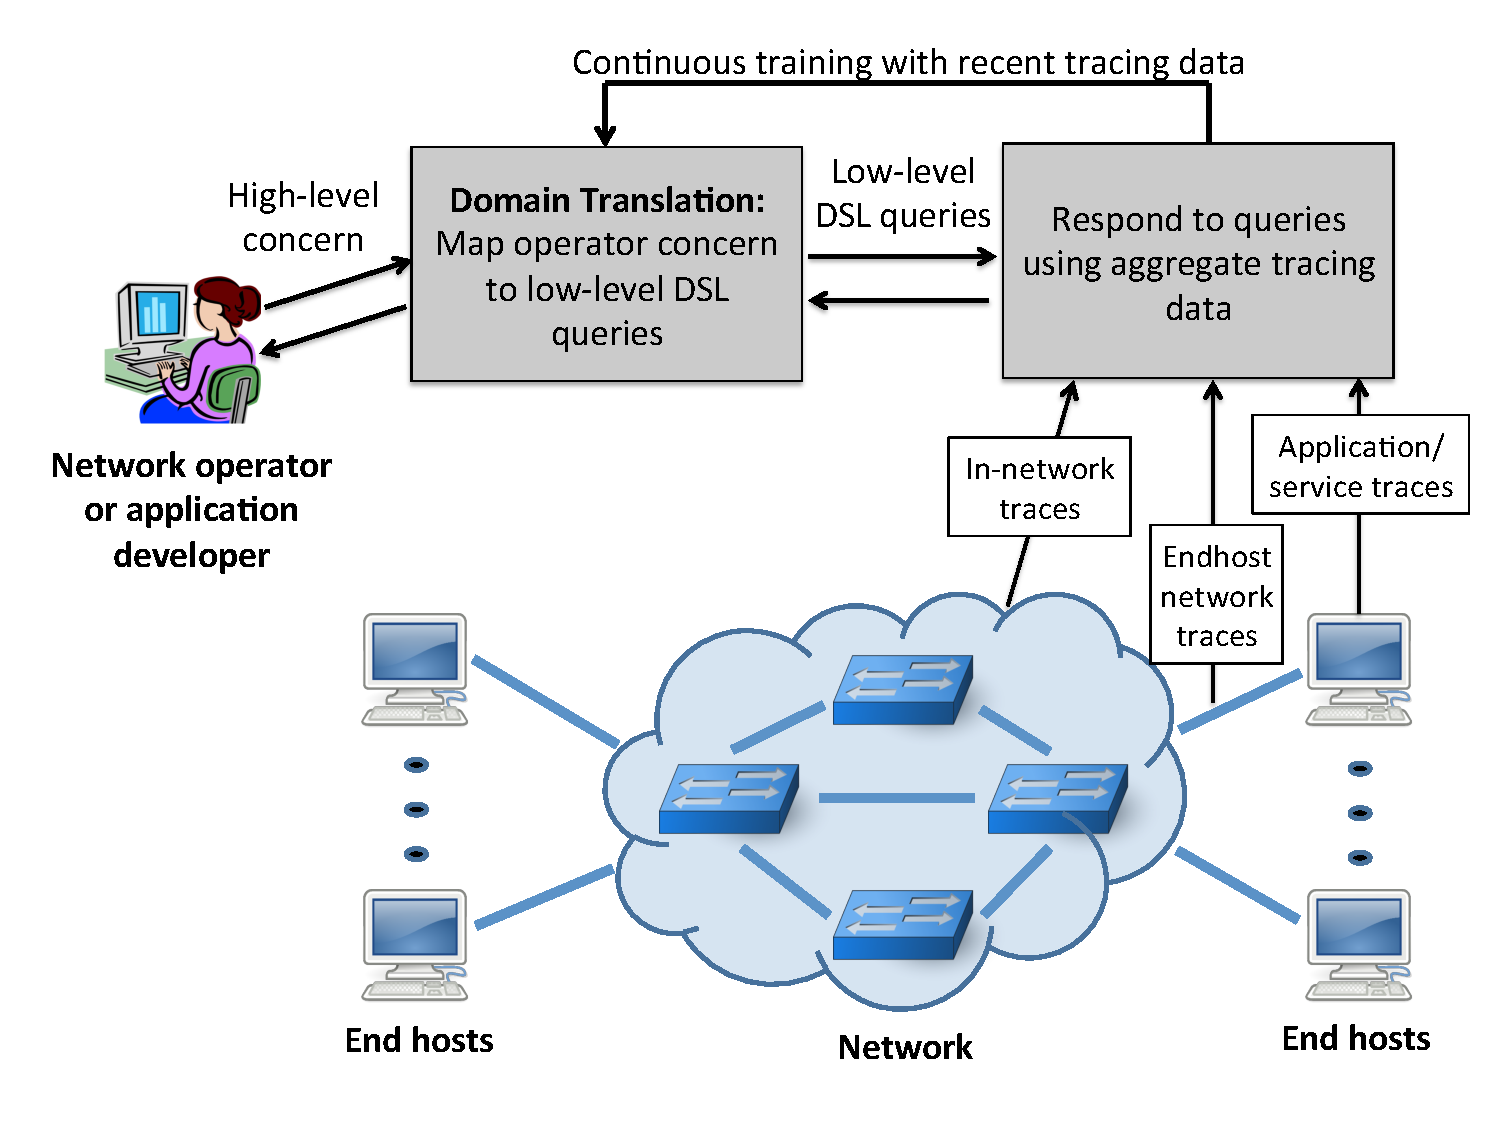
\includegraphics[width=0.7\textwidth]{tracing_figure.pdf}
\caption{Overview of our proposal to automatically bridge the gap between
operator/developer concerns and low-level tracing systems.}
\label{fig:overview}
\end{figure*}

In this proposal, we seek to bridge the gap between low-level debugging systems
and high-level operator concerns. In particular, our aim is to enable
developers to specify high-level concerns and automatically receive actionable
responses; the process of converting high-level concerns to DSL queries
encompassing application, endhost, and in-network debuggers will be automated
and hidden from developers and operators. Mapping high-level concerns to DSLs
can be done in one of two ways: 1) using tracing data which was collected
during the execution in question, or 2) assuming that all possible tracing data
is available. The former can use already collected data to provide a fast
response, but may restrict the set of possible DSL queries, potentially
affecting the response quality. In contrast, the latter approach isolates DSL
query generation from the available data, ensuring that the optimal queries are
considered; however, collecting the necessary data may be challenging as
execution environments are difficult to reproduce. We plan to explore this tradeoff
in more detail using concrete environments and real tracing data.

With either approach for generating DSL queries, a key challenge is to figure
out how to partition a potentially ambiguous high-level concern into the
appropriate DSLs. Prior systems have attempted to partition program logic
across different network domains~\cite{snap,maple}. However, these systems are designed
to receive well-formed inputs (often expressed with a separate DSL), and
partition logic across domains whose relationships are well understood (i.e., the
control plane and the data plane). In contrast, our proposal may be presented
with loosely-formed, high level concerns. In addition, we must map those
concerns to cooperative DSL queries across environments that are largely dynamic
and have been mostly treated in isolation to date.

To overcome these challenges, we propose two solutions. First, we plan to
employ Natural Language Processing techniques to bridge query abstraction
levels by mapping high-level operator concerns to DSL queries.  Second, we will
use tracing data collected at each point in the ecosystem (i.e., applications,
endhosts, and networks) to generate a model which relates low-level operations,
tracing data, and DSL queries across domains. Given the dynamic nature of the
end-to-end environment in terms of workloads, configurations, and available
data, we propose that each component is continually trained to update its model
with the latest tracing data. For example, training can use techniques like
LSTM to prioritize recently observed tracing data without forgetting past
(potentially sporadic) events~\cite{concode}. Figure~\ref{fig:overview} depicts
our proposed workflow.

Several properties of modern networks and distributed systems complicate this
vision. First, how can we support broad sets of loosely-formed queries? Prior
systems have attempted to automatically parse trouble tickets using NLP
techniques based on fixed keywords and input structures~\cite{netsieve}. In
order to support arbitrary queries from each part of the ecosystem, we plan to
develop models which relate keywords in each domain based on causal actions
observed in the collected traces.  Second, how can we collect sufficient
training data to cover the wide range of possible developer queries.  In
addition to training with actual snapshot data from prior execution and bug
reports, we plan to generate synthetic training data to highlight potential
issues (e.g., resource contention, race conditions, etc.).  Third, prior
systems have shown that collecting comprehensive tracing data at any one part
of a networked system poses scaling challenges, both for storage and
processing~\cite{pathqueries,demi}. Our proposal requires the aggregation of
tracing data from each part of the ecosystem. Because the importance of
collected data is most effectively considered in aggregate, we must develop
efficient pruning strategies that can scalably collect the important tracing
information without sacrificing insights.  Fourth, how can we handle
information gaps in the ecosystem due to privacy concerns over tracing data or
lack of administrative cooperation? Our models must be robust to varying
amounts of contextual data and misreported tracing data.

%In light of these challenges, we plan
%to keep the developer in the loop of the query generation process. In this way,
%developers may be able to provide additional information to tune intermediate
%representations that they still have familiarity with.

Prior work has proposed using machine learning for classification to associate
network-specific queries with tracing data from single
machines~\cite{netpoirot}. Our proposal differs from these approaches in two
key ways. First, we propose using machine learning in part as a language
translation tool, connecting the abstract, high-level developer language to the
low-level, structured query languages that existing tracing systems support.
Debugging systems have continually tried to raise the level of abstractions for
queries and user interfaces. 
% However, in order to go the next step and connect
% every part of the ecosystem, we believe that tackling the unstructured concerns
% of operators is the next challenge. 
Second, our proposed model that relates DSL
queries (and the corresponding tracing data) is not restricted to a single
machine that is controlled by one administrative entity. Instead, we plan to
merge data and DSL queries across different combinations of applications,
machines, and networks, in order to accurately respond to high-level developer
concerns with actionable suggestions.


